% LaTeX figure environment for the ResNet18 clean-qualified multi-seed
% fall-recall-vs-epsilon plot.
% Image: results/cross_architecture/resnet/figures/resnet18_clean_qualified_fall_recall_vs_epsilon.png
% Source data commits: seed42 3578136, seed43 5024193, seed44 dd3460b, seed46 9cf6172
% (seed45 6db1485 NON-CONVERGED, excluded). Requires \usepackage{graphicx}.

\begin{figure}[t]
  \centering
  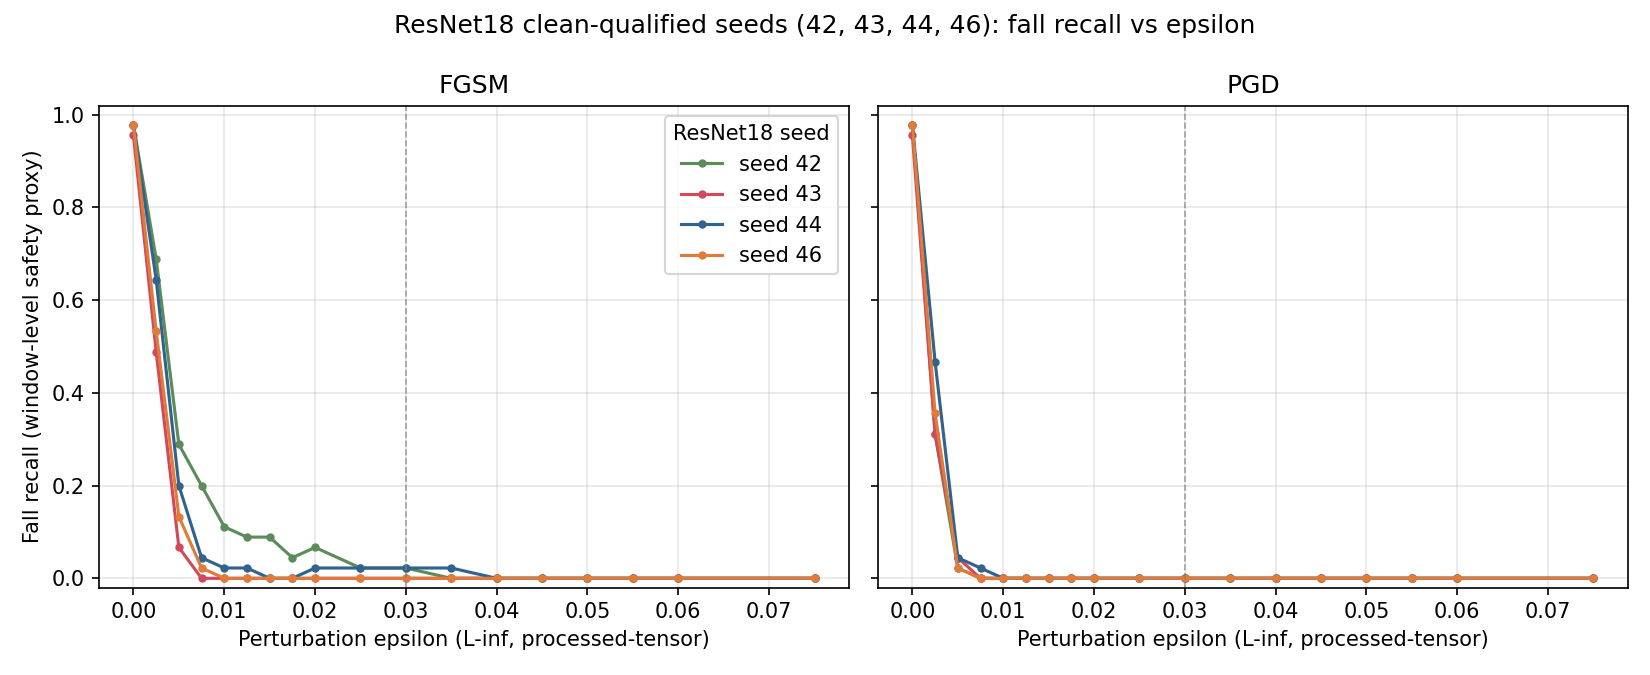
\includegraphics[width=\linewidth]{results/cross_architecture/resnet/figures/resnet18_clean_qualified_fall_recall_vs_epsilon.png}
  \caption[ResNet18 clean-qualified multi-seed fall recall vs.\ perturbation budget]{%
    ResNet18 multi-seed fall recall versus $L_\infty$ perturbation budget
    $\varepsilon$ for the four clean-qualified seeds (42, 43, 44, 46), shown as
    separate FGSM (left) and PGD (right) panels. Each curve is one seed on the
    held-out test split ($n=500$ windows, $45$ fall windows); the dashed vertical
    line marks the matched evaluation point $\varepsilon=0.03$. Perturbations are
    digital-domain, processed-tensor perturbations, not physical-layer or
    over-the-air attacks. All four clean-qualified seeds lose essentially all fall
    recall under PGD by $\varepsilon\le0.010$ and reach $0.000$ fall recall under
    PGD at $\varepsilon=0.03$. Seed~45 is excluded as a non-converged training run
    (it appears in the convergence-status table only). This is a ResNet18
    multi-seed result over clean-qualified seeds, not a multi-seed
    cross-architecture reliability claim.}
  \label{fig:resnet18-multiseed-fall-recall}
\end{figure}
